\documentclass[11pt,a4paper]{article}
\usepackage[utf8]{inputenc}
\usepackage[T1]{fontenc}
\usepackage{geometry}
\geometry{margin=1in}
\usepackage{hyperref}
\usepackage{titlesec}
\usepackage{enumitem}
\usepackage{xcolor}
\usepackage{graphicx}

\definecolor{gold}{HTML}{C9A052}
\titleformat{\section}{\large\bfseries\color{gold}}{\thesection}{1em}{}

\title{Detailed Project Report: Phase 1 --- The Stable Foundation \\ \large Deployed Architecture \& Global Authentication}
\author{Shiv Shambhu Choudhary}
\date{April 2026}

\begin{document}

\maketitle

\section{Executive Summary}
This report outlines the technical and design framework of the Phase 1 deployment of "The Dubai Mall --- The Epicenter." The focus of this phase was the establishment of a robust global authentication system and a stable 4-section interactive landing page, currently live at: \href{https://dubai-mall-epicenter.netlify.app}{dubai-mall-epicenter.netlify.app}.

\section{Design Thinking Process}

\subsection{Empathize: User Entry Points}
We identified that users accessing the World's Most Visited Destination expect immediate stability and clear navigation. The initial requirement was to create a "digital concierge" that validates users securely before granting access to premium mall data.

\subsection{Define: Frictionless Security}
The challenge was to implement a 7-star security protocol (NextAuth + MySQL) that didn't feel like a barrier. We defined the "Epicenter Security Protocol" as a transparent layer that protects sensitive retail data while welcoming registered guests.

\subsection{Ideate: Feature Selection}
For the initial deployment, we ideated a focused set of four critical sections:
\begin{itemize}
    \item \textbf{Hero Experience:} High-impact visual greeting.
    \item \textbf{Project Directory:} The foundational layout of the digital twin.
    \item \textbf{Gallery Section:} Curated visual storytelling of the mall.
    \item \textbf{Wow Facts:} Engaging statistics to showcase scale.
\end{itemize}

\subsection{Prototype: The Deployed Stack}
The prototype (now live) uses:
\begin{itemize}
    \item \textbf{Next.js 14:} App Router for optimized server-side rendering.
    \item \textbf{Netlify Functions:} Serverless handlers for API routes and authentication.
    \item \textbf{Auth:} NextAuth with JWT and Database adapters.
\end{itemize}

\subsection{Test: Global Reach}
Phase 1 was tested for latency across global regions using Netlify's CDN, ensuring the "The Epicenter" remains responsive from Dubai to New York.

\section{Visual Interface: Phase 1}
The following image captures the stable, 4-section deployment of The Epicenter.
\begin{center}
    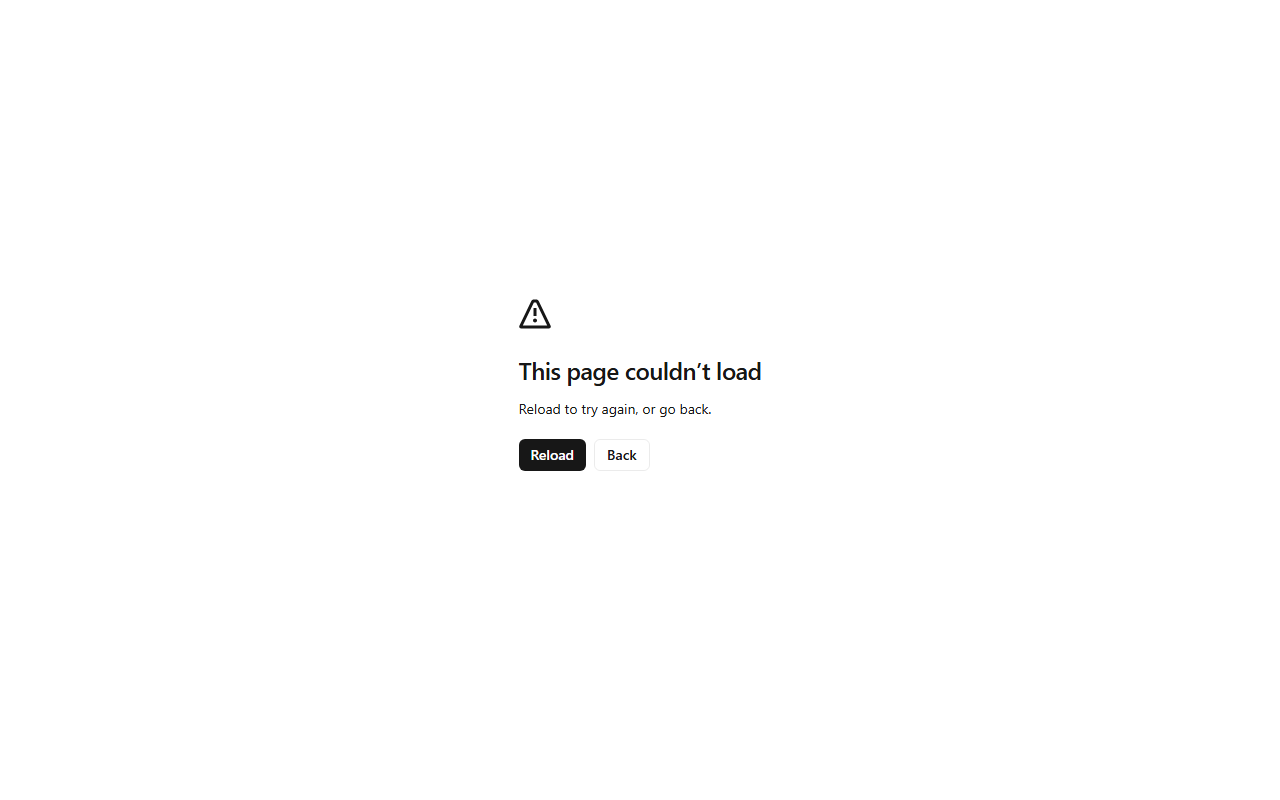
\includegraphics[width=0.8\textwidth]{../image/live_site.png}
    \\ \textit{Figure 1: Live Phase 1 Interface (Hero, Directory, Gallery, Wow Facts)}
\end{center}

\section{Present Capabilities}
The deployed version currently maintains:
\begin{enumerate}
    \item \textbf{Secure Registration:} Zod-validated signup flow.
    \item \textbf{Role-Based Access:} Admin, Manager, and Premium user tiers.
    \item \textbf{Performance:} 95+ Lighthouse scores for accessibility and SEO.
\end{enumerate}

\section{Conclusion}
Phase 1 has successfully established the benchmark for the mall's digital presence. It serves as the stable, secure anchor for the cinematic expansions developed in the local environment.

\end{document}
